\section{Laboratory work implementation}

\subsection{Tasks and Points}

\textbf{Advanced Level (nota 9 || 10):}\\
\indent 
- seteaza un branch to track a remote origin pe care vei putea sa faci push (ex. Github, Bitbucket or custom server)\\
\indent 
- reseteaza un branch la commit-ul anterior\\
\indent 
- merge 2 branches\\
\indent 
- rezolvarea conflictelor a 2 branches\\
\indent 
\textbf{Bonus Point:}\\
\indent 
- Scrie un script care va compila HelloWolrdPrograms projects.\\
\indent 

\subsection{Analiza lucrarii de laborator}
\selectlanguage{russian}

Ссылка на репозиторий https://github.com/IanaPushcash/MIDPS.\\
\indent 
В первой части лабораторной работы нами был создан репозиторий на сервере githab.com. Далее с ним была связана папка на нашем компьютере и идентифицирован ключ SSH.\\\\
\indent 

\begin{figure}[h]
	\center{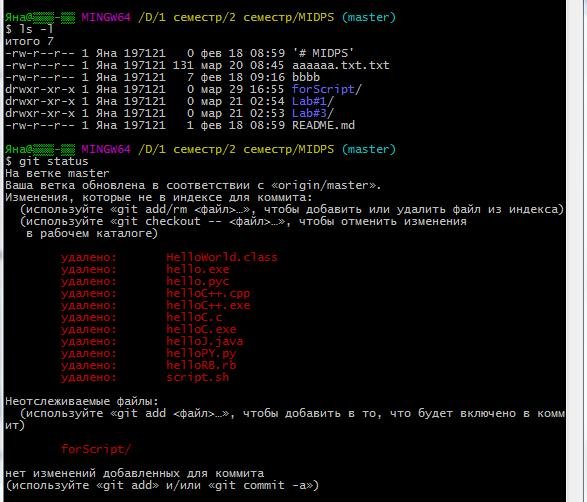
\includegraphics[width=0.8\linewidth]{images/1.jpg}}
	\caption{Проверим состояние репозитория.}
	\label{ris:image}
\end{figure}
\hfill
\begin{figure}[h]
	\center{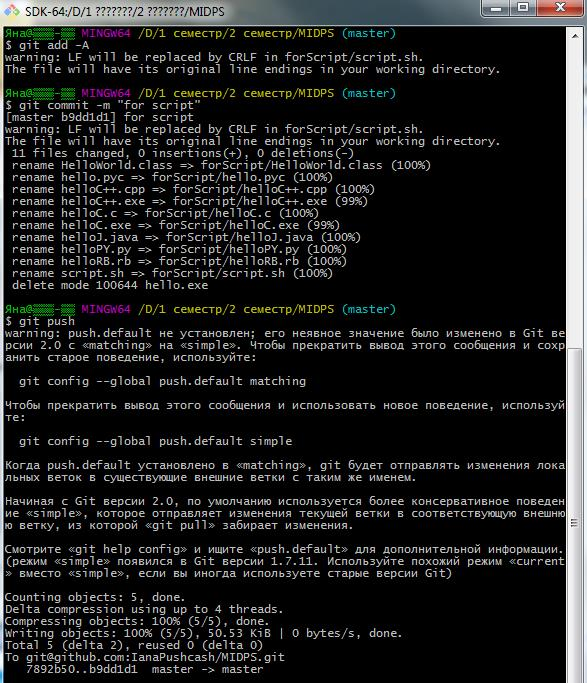
\includegraphics[width=0.8\linewidth]{images/2.jpg}}
	\caption{Добавим изменения на индексирование. Закомментируем изменения. Загрузим на репозиторий.}
	\label{ris:image}
\end{figure}
\hfill
\begin{figure}[h!]
	\center{
\includegraphics[width=0.8\linewidth]{images/3.jpg}}
	\caption{Проверим состояние репозитория.}
	\label{ris:image}
\end{figure}
\hfill
\begin{figure}[h!]
	\center{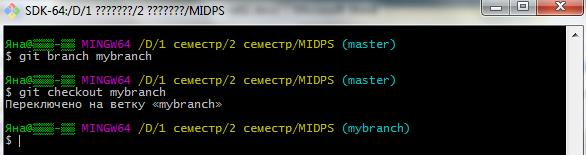
\includegraphics[width=0.8\linewidth]{images/4.jpg}}
	\caption{Создадим новую ветвь и перейдем на неё.}
	\label{ris:image}
\end{figure}
\hfill
\begin{figure}[h]
	\center{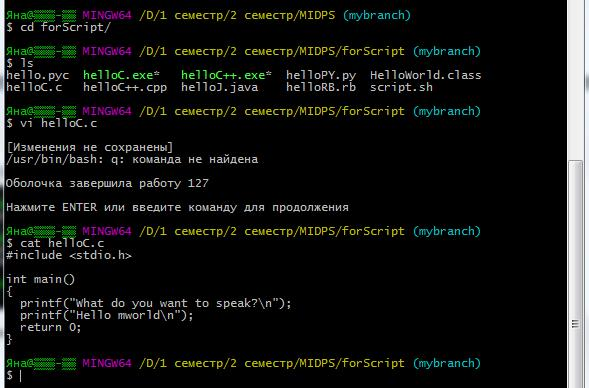
\includegraphics[width=0.8\linewidth]{images/5.jpg}}
	\caption{Изменим один из файлов в репозитории, создав этим конфликт.}
	\label{ris:image}
\end{figure}
\hfill
\begin{figure}[h]
	\center{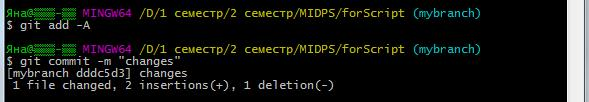
\includegraphics[width=0.8\linewidth]{images/6.jpg}}
	\caption{Добавим изменения на репозиторий.}
	\label{ris:image}
\end{figure}
\hfill
\begin{figure}[h]
	\center{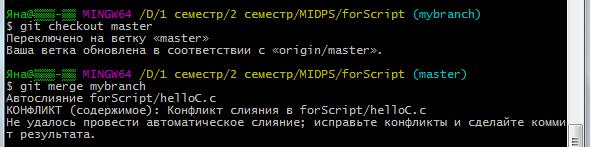
\includegraphics[width=0.8\linewidth]{images/7.jpg}}
	\caption{Вернемся на основную ветвь и соединим обе ветви.}
	\label{ris:image}
\end{figure}
\hfill
\begin{figure}[h]
	\center{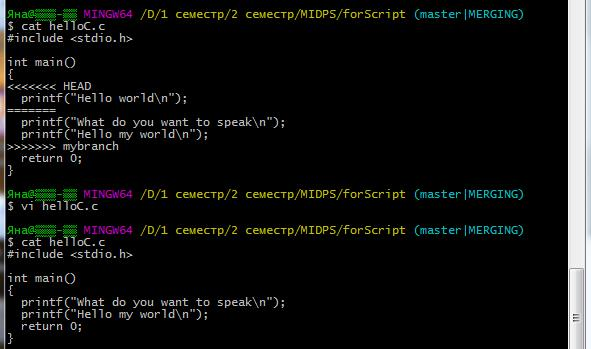
\includegraphics[width=0.8\linewidth]{images/8.jpg}}
	\caption{Просматриваем и исправляем конфликт.}
	\label{ris:image}
\end{figure}
\hfill
\begin{figure}[h]
	\center{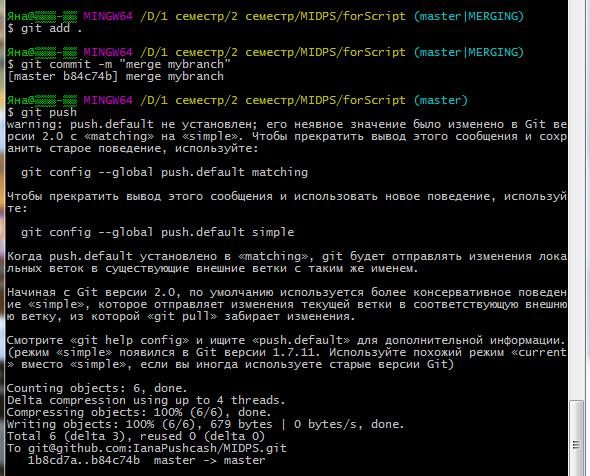
\includegraphics[width=0.8\linewidth]{images/9.jpg}}
	\caption{Добавляем изменения на репозиторий.}
	\label{ris:image}
\end{figure}
\hfill
\begin{figure}[h!]
	\center{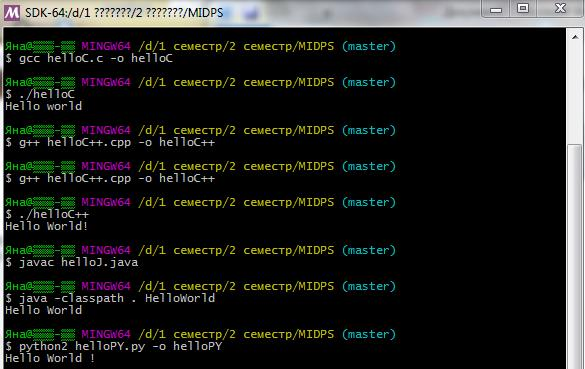
\includegraphics[width=0.8\linewidth]{images/10.jpg}}
	\caption{Напишем скрипт для компиляции программ через Git Bash.
		Для этого подключим необходимые библиотеки и  PATH. Для java прописываем export PATH=\$PATH:"/C/Program Files/Java/jdk1.8.0\_60/bin/".}
	\label{ris:image}
\end{figure}
\hfill
\begin{figure}[h]
	\center{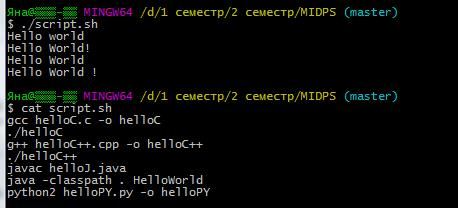
\includegraphics[width=0.8\linewidth]{images/11.jpg}}
	\caption{Объединим все команды в один скрипт.}
	\label{ris:image}
\end{figure}
\hfill

\clearpage